\chapter{إنشاء نافذة و مساحات}

في الفصل السابق، قمنا بالإلمام حول أهم المميزات التي تمنحها المكتبة 
\textenglish{SDL}.
يجدر بك أن تكون قد ثبتّ المكتبة، و تعلّمت كيفية إنشاء مشروع جديد يشتغل بشكل جيد.  على الرغم من أنّه كان فارغا.

سندخل في مضمون موضوعنا في هذا الفصل. سنقوم بتطبيق أساسيات لغة الـ\textenglish{C}
مع
\textenglish{SDL}.
كيف يتم تحميل الـ\textenglish{SDL} ؟
كيف يتم فتح نافذة بالأبعاد التي نريد ؟ كيف نرسم داخل النافذة ؟

لدينا أمور كثيرة لنعرفها، فهيّا بنا !

\section{تحميل و إيقاف الـ\textenglish{SDL}}

العديد من المكتبات المكتوبة بلغة الـ\textenglish{C}،
تستلزم أن يتم تحميلها ثم غلقها حين ننتهي منها، و ذلك لاستعمال دوال محددة. المكتبة
\textenglish{SDL}
من بين هذه المكتبات. 

بالفعل، فالمكتبة تحتاج أن يتم تحميل عدد معيّن من المعلومات إلى الذاكرة العشوائية لتستطيع أن تشتغل بشكل صحيح. يتم هذا التحميل بشكل حيّ باستعمال الدالة 
\InlineCode{malloc}
(إنّها مهمّة جدّا هنا !). و كما تعلم فإن قلت
\InlineCode{malloc}،
سأقول كذلك
\InlineCode{free} !\\
يجب عليك تحرير الذاكرة التي حجزتها و لم تعد بحاجة إليها. إن لم تفعل، فالبرنامج يمكن أن يأخذ حيّزاً كبيراً من الذاكرة بدون فائدة، و يمكن لذلك أحيانا أن يدرّ بنتائج كارثية. تخيّل القيام بحلقة غير منتهية من
\InlineCode{malloc}
دون قصد، في بضع ثوان ستسدّ كلّ الذاكرة !

هاهما الدالتان الأولتان الخاصّتان بالـ\InlineCode{SDL}
اللتان يجب عليك أن تعرفهما :
\begin{itemize}
	\item \InlineCode{SDL\_Init} :
	تحميل المكتبة في الذاكرة العشوائية (باستخدام الـ\InlineCode{malloc}).
	\item \InlineCode{SDL\_Quit} :
	تحرير المكتبة من الذاكرة (باستعمال الـ\InlineCode{free}).
\end{itemize}

أي أن أوّل شيء يجب أن تقوم به في البرنامج هو استدعاء
\InlineCode{SDL\_Init}،
و آخر شيء هو استدعاء
\InlineCode{SDL\_Quit}.

\subsection{\texttt{SDL\_Init} : تحميل المكتبة \textenglish{SDL}}

الدالة
\InlineCode{SDL\_Init}
تستقبل معاملا. إذ يجب أن يتم تحديد أي جزء من المكتبة نريد تحميله.

\begin{question}
آه حقّا ! هل الـ\textenglish{SDL}
تتكون من كثير من الأجزاء ؟
\end{question}

نعم بالطبع ! فهناك جزء من المكتبة يتعامل مع الشاشة، و آخر يتعامل مع الصوت، إلخ.

توفّر لنا المكتبة عدداً من الثوابت التي تسمح لنا بتحديد اسم الجزء الذي نريد تحميله من المكتبة.

\begin{Table}{2}
الثابت & الشرح \\
\texttt{SDL\_INIT\_VIDEO} &
تحميل الجزء الخاص بالعرض (الفيديو)، إنه الجزء الذي نحمله غالباً.\\
\texttt{SDL\_INIT\_AUDIO} &
تحميل الجزء الخاص بالصوت، هذا ما يسمح لك مثلا بتشغيل الموسيقى مثلا.\\
\texttt{SDL\_INIT\_CDROM} &
تحميل الجزء الخاص بقارئ القرص المضغوط، و ذلك للتحكم به.\\
\texttt{SDL\_INIT\_JOYSTICK} &
تحميل الجزء الخاص بجهاز التحكم 
\textenglish{Joystick}.\\
\texttt{SDL\_INIT\_EVERYTHING} &
تحميل كل الأجزاء التي ذكرتها سابقا.\\
\end{Table}

إذا استدعيت الدالة بهذا الشكل

\begin{Csource}
SDL_Init(SDL_INIT_VIDEO);
\end{Csource}

فإن نظام العرض سيتم تحميله في الذاكرة، فيمكنك أن تفتح نافذة و ترسم فيها، إلخ.\\
كل ما قمنا به هو إعطاء عدد إلى الدالة 
\InlineCode{SDL\_Init}
بالاستعانة بثابت. أنت لا تعرف أي عدد هو، و هذا أمر جيد. إذ أنك غير مجبر على حفظ العدد، بل التعبير عنه باسم الثابت فقط. 

الدالة 
\InlineCode{SDL\_Init}
تقرأ العدد و هكذا تحدد الأنظمة الواجب تحميلها.

الآن لو تكتب :

\begin{Csource}
SDL_Init(SDL_INIT_EVERYTHING);
\end{Csource}

ستقوم بتحميل كل أنظمة الـ\textenglish{SDL}،
لا تقم بهذا إلا في حالة كنت بالفعل تحتاج إلى كلّ شيء، ليس جيداً إثقال الحاسوب بوحدات لا فائدة منها.

\begin{question}
ماذا لو أردت تحميل الصوت و الفيديو فقط. هل يجدر بي استخدام
\InlineCode{SDL\_INIT\_EVERYTHING} ؟
\end{question}

لن تستعمل
\InlineCode{SDL\_INIT\_EVERYTHING}،
من أجل تحميل وحدتين، هذا جنون ! لحسن الحظ، يمكننا تجميع الخيارات بواسطة الرمز
\InlineCode{|}.

\begin{Csource}
// Loading the video and the audio
SDL_Init(SDL_INIT_VIDEO | SDL_INIT_AUDIO);
\end{Csource}

كما يمكنك وضع ثلاثة دون مشاكل :

\begin{Csource}
// Loading the video, the audio and the timer
SDL_Init(SDL_INIT_VIDEO | SDL_INIT_AUDIO | SDL_INIT_TIMER);
\end{Csource}

\begin{information}
هذه "الخيارات" التي نبعثها للدالة 
\InlineCode{SDL\_Init}
نسميها بـ\textit{الأعلام}
(\textenglish{Flags}).
هذه الكلمة نستعملها كثيراً في علوم الحاسوب.\\
تذكّر إذا أن الإشارة
\InlineCode{|}
خاصة بدمج الخيارات. إنها تشبه الإضافة إلى حدّ ما.
\end{information}

\subsection{\texttt{SDL\_Quit} : إيقاف المكتبة \textenglish{SDL}}

هذه الدالة سهلة الاستعمال لأنها لا تحتاج إلى أي معامل :

\begin{Csource}
SDL_Quit();
\end{Csource}

كل الأنظمة سيتم إيقافها و يتم تحرير الذاكرة.\\
باختصار، هذه الدالة أداة للخروج من المكتبة بشكل نظيف، و لنقل للخروج من برنامجك.

\subsection{نموذج عن برنامج \textenglish{SDL}}
باختصار، هذا ما يبدو عليه برنامج
\textenglish{SDL}
في نسخته الأبسط :

\begin{Csource}
#include <stdlib.h>
#include <stdio.h>
#include <SDL/SDL.h>
int main(int argc, char *argv[])
{
	SDL_Init(SDL_INIT_VIDEO); // Starting the SDL (Here we load the video system)
	SDL_Quit(); // Stopping the SDL (Freeing the memory).
	return 0;
}
\end{Csource}

هذا نموذج عن برنامج بسيط، عبارة عن مخطط لبرامج
\textenglish{SDL}
التي نكتبها. في الواقع، البرنامج الحقيقي يكون ممتلأً كثيرا إذ يحتوي عدّة استدعاءات لدوال، تقوم بدورها بمزيد من الاستدعاءات.\\
الأمر المهمّ في النهاية، هو أنّ
\textenglish{SDL}
يجب أن تُحمّل في البداية و تُغلق عندما لا تصبح بحاجة إليها.

\subsection{معالجة الأخطاء}

الدالة 
\InlineCode{SDL\_Init}
تقوم بإرجاع قيمة :

\begin{itemize}
	\item $ -1 $ : في حال وجود خطأ.
	\item $ 0 $ : في حالة عدم وجود أي خطأ.
\end{itemize}

لست مجبراً، لكن يمكنك اختبار القيمة المُرجعة. قد تكون طريقة جيّدة لمعالجة الأخطاء في برنامجك، و هذا ما سيساعدك على حلّها.

\begin{question}
لكن كيف أقوم بإظهار الخطأ الحادث ؟
\end{question}

سؤال وجيه ! ليس لدينا كونسول الآن، كيف نخزّن و نعرض رسائل الخطأ ؟

هناك حلّان :
\begin{itemize}
	\item يمكننا التعديل على خاصيات المشروع، لكي نسمح له باستعمال الكونسول أيضاً. سنتمكّن في هذه الحالة من استخدام الدالة 
	\InlineCode{printf})،
	\item أو نكتب الأخطاء في ملف. تستخدم الدالة
	\InlineCode{fprintf}.
\end{itemize}

لقد اخترت أن نكتب في ملف. و بهذا فإن العمل على ملف يحتاج إلى فتح هذا الأخير بـ\InlineCode{fopen}
و غلقه بـ\InlineCode{fclose}،
و الأمر أقلّ سهولة من استعمال الـ\InlineCode{printf}.\\
لحسن الحظ، هناك طريقة أسهل و هي استعمال مخرج الأخطاء القياسي.

يوجد متغير 
\InlineCode{stderr}
معرّف في 
\InlineCode{stdio.h}
يقوم بالتأشير نحو المنطقة التي يُمكن أن يُكتب فيها الخطأ. غالبا في الويندوز، هذه المنطقة عبارة عن ملف يحمل الاسم 
\InlineCode{stderr.txt}.
بينما في اللينكس فإن الأخطاء غالباً ما يتم إظهارها على الكونسول. هذا المتغير يتم إنشاؤه تلقائيّا في بداية البرنامج و يتم حذفه في نهايته، أي أنك لست مجبراً على استعمال 
\InlineCode{fopen}
و
\InlineCode{fclose}.\\
يمكنك استعمال الدالة
\InlineCode{fprintf}
على 
\InlineCode{stderr}
بدون استعمال  
\InlineCode{fopen}
و 
\InlineCode{fclose} :

\begin{Csource}
#include <stdlib.h>
#include <stdio.h>
#include <SDL/SDL.h>
int main(int argc, char *argv[])
{
	if (SDL_Init(SDL_INIT_VIDEO) == -1) // Starting the SDL, if there's an error :
	{
		fprintf(stderr, "Error while initializing SDL : %s\n", SDL_GetError()); // Writing the error
		exit(EXIT_FAILURE); // We exit the program
	}
	SDL_Quit();
	return EXIT_SUCCESS;
}
\end{Csource}

ما الجديد في هذه الشفرة المصدرية ؟

\begin{itemize}
	\item لقد كتبنا الخطأ الذي وجدناه في
	\InlineCode{stderr}.
	الرمز 
	\InlineCode{\%s}
	يسمح للـ\textenglish{SDL} 
	بالإشارة إلى تفاصيل الخطأ : الدالة 
	\InlineCode{SDL\_GetError}
	في الحقيقة تقوم بإرجاع آخر خطأ
	\textenglish{SDL}.
	\item نخرج باستعمال الـ\InlineCode{exit()}.
	لحدّ الآن لا يوجد شيء جديد مقارنة بما جرت العادة، ستلاحظ أنني استعمل الثابت 
	\InlineCode{EXIT\_FAILURE}
	كقيمة يقوم البرنامج الرئيسي بإرجاعها، بينما استعملت في النهاية الثابت 
	\InlineCode{EXIT\_SUCCESS}
	في مكان الـ0.\\
	ما الذي قمت به ؟ لقد قمت بتحسين الطريقة التي تعودنا أن نكتب بها الشفرة. لقد استخدمت اسم الثابت الّذي يعني "خطأ" و الذي هو نفسه بالنسبة لجميع أنظمة التشغيل. بينما الأعداد تختلف من نظام إلى آخر.\\
	لهذا فإن الملف
	\InlineCode{stdlib.h}
	تسمح باستعمال ثابتتين (معرّفي 
	\InlineCode{\#define}) :
	
	\begin{itemize}
		\item \InlineCode{EXIT\_FAILURE} :
		قيمة يتم إرجاعها في حالة وجود خطأ ما في البرنامج.
		\item \InlineCode{EXIT\_SUCCESS} :
		قيمة يتم إرجاعها في حالة عدم وجود أي خطأ.
	\end{itemize}
	
	باستعمال أسماء الثوابت بدلاً من قيمها، ستضمن بأنك قد بعثت القيمة الصحيحة.\\
	لماذا ؟ لأن الملف
	\InlineCode{stdlib.h}
	يتغيّر حسب نظام التشغيل الّذي أنت عليه، لذا فقيم الثوابت ستتأقلم مع النظام من دون أنّ نحتاج إلى تغيير شيء !  و هذا ما يجعل لغة الـ\textenglish{C}
	متوافقة مع كلّ أنظمة التشغيل (بافتراض أنّك تبرمج بالطريقة الصحيحة باستخدام الأدوات المتوفّرة، كما فعلنا هنا).

\begin{information}
	استعمال أسماء الثوابت لا يعود علينا بكثير من النفع الآن، لكن من الأحسن استعمالها. سنقوم بذلك انطلاقاً من الآن.
\end{information}
\end{itemize}

\section{فتح نافذة}

حسناً، لقد تم فتح و غلق المكتبة بنجاح. الخطوة التالية التي يريد تعلّمها الجميع هي كيفية فتح نافذة ! 

لكي نبدأ، تأكد من أن لديك
\InlineCode{main}
تشبه هذه :

\begin{Csource}
int main(int argc, char *argv[])
{
	if (SDL_Init(SDL_INIT_VIDEO) == -1)
	{
		fprintf(stderr, "Error while initializing SDL");
		exit(EXIT_FAILURE);
	}
	SDL_Quit();
	return EXIT_SUCCESS;
}
\end{Csource}

هذه هي حالتك لو اتبعت جيداً من بداية الفصل. حاليّا، كلّ ما سنقوم بتحميله هو نظام العرض
(\InlineCode{SDL\_INIT\_VIDEO})،
هذا ما يهمّنا.
\subsection{اختيار وضع العرض}

أول شيء نقوم به بعد 
\InlineCode{SDL\_Init}،
هو تحديد وضع العرض الذي نريد استعماله، أي الدقة
(\textenglish{Resolution})،
عدد الألوان بالإضافة إلى خصائص أخرى.

من أجل هذا سنستعمل الدالة
\InlineCode{SDL\_SetVideoMode}
التي تستقبل 4 معاملات :

\begin{itemize}
	\item عرض النافذة التي نريدها
	(\textenglish{pixels})،
	\item طول النافذة التي نريدها
	(\textenglish{pixels})،
	\item عدد الألوان القابلة للعرض
	(\textenglish{bits/pixel})،
	\item الخيارات (الأعلام).
\end{itemize}

لا أعتقد أن طول و عرض النافذة يحتاجان إلى شرح، بينما عدد الألوان و الأعلام هما المعاملان الأكثر أهميّة.

\begin{itemize}
	\item \textbf{عدد الألوان} : 
	هو العدد الأقصى للألوان التي يمكن أن تظهر في النافذة. إن كنت من عشاق ألعاب الفيديو، ستكون معتاداً على هذا الأمر. فإن قيمة 
	\textenglish{32 bits/pixel}
	تسمح بإظهار ملايير الألوان، بينما إنه من الممكن أن نختار قيمة أقل كـ\textenglish{16 bits/pixel}
	(تسمح بعرض 65536 لون) أو حتى 
	\textenglish{8 bits/pixel}
	(تسمح بعرض 256 لون مختلف)، هذا الأمر مفيد حينما تريد برمجة تطبيقات من أجل جهاز بسيط كالـ\textenglish{PDA}
	أو الهاتف المحمول.
	\item الخيارات : تماما مثل الـ\InlineCode{SDL\_Init}،
	علينا باستعمال أعلام من أجل تعريف خصائص. هذه أهم الأعلام التي يمكنك استعمالها (يمكنك استعمال العديد منها، يتم التفريق بينها باستعمال الرمز
	\InlineCode{|}) :
	\begin{itemize}
		\item \InlineCode{SDL\_HWSURFACE} :
المعطيات سيتم حفظها في في الذاكرة الرسومية للبطاقة
\textenglish{3D}.
الشيء الجيد : إنها الذاكرة الأكثر سرعة. الشيء السيّء : يصعب إيجاد مساحة شاغرة في هذا النوع من الذاكرة مقارنة بالأخرى 
(\InlineCode{SDL\_SWSURFACE}).
		\item \InlineCode{SDL\_SWSURFACE} :
المعطيات يتم حفظها في ذاكرة النظام (أي في الـ\textenglish{RAM})،
الشيء الجيد : يوجد الكثير من المكان في هذه الذاكرة. الشيء السيء : أقل سرعة و أقل كفاءة.
		\item \InlineCode{SDL\_RESIZABLE} :
		ستصبح مقاييس أبعاد النافذة قابلة للتعديل، لأنها ليست كذلك تلقائيا.
		\item \InlineCode{SDL\_NOFRAME} :
		لن يصبح للنافذة أية حواش أو شريط علوي لكتابة عنوان النافذة.
		\item \InlineCode{SDL\_FULLSCREEN} :
		نمط الشاشة الكاملة. لن تستطيع رؤية أية نافذة أخرى لأن نافذة البرنامج الحالي تهيمن على كلّ الشاشة، مع تعديل دقّة الشاشة في حالة الضرورة.
		\item \InlineCode{SDL\_DOUBLEBUF} : وضع 
		\textenglish{double buffering}،
		تقنية مستعملة بكثرة في برمجة الألعاب ثنائية الأبعاد. تقضي بأن يكون تحرّك الأشياء على الشاشة مرناً، لأنه إن لم يكن كذلك، سيكون التحرّك سيئاً، سأشرح هذا الأمر بالتفصيل لاحقاً.
	\end{itemize}
\end{itemize}

إذا كتبت الشفرة المصدرية التالية :

\begin{Csource}
SDL_SetVideoMode(640, 480, 32, SDL_HWSURFACE);
\end{Csource}

فإنه سيقوم بفتح نافذة ذات أبعاد
$640 \times 480$،
 و بعدد ألوان
\textenglish{32 bits/pixel}
(ملايير الألوان)، و ستم تحميل النافذة على الذاكرة الرسوميّة (إنّها الأسرع، لذلك نفضّل استعمالها).

كمثال آخر، لو نأخذ :

\begin{Csource}
SDL_SetVideoMode(400, 300, 32, SDL_HWSURFACE | SDL_RESIZABLE | SDL_DOUBLEBUF);
\end{Csource}

هذه الشفرة تفتح نافذة مقاييس  أبعادها قابلة للتعديل، بأبعاد ابتدائية 
$400 \times 300$،
و بعدد ألوان 
\textenglish{32 bits/pixel}
كما أن تقنية 
\textenglish{double buffering}
مفعّلة.

هذه أوّل شفرة مصدرية بسيطة يمكنك تجريبها :

\begin{Csource}
#include <stdlib.h>
#include <stdio.h>
#include <SDL/SDL.h>
int main(int argc, char *argv[])
{
	SDL_Init(SDL_INIT_VIDEO);
	SDL_SetVideoMode(640, 480, 32, SDL_HWSURFACE);
	SDL_Quit();
	return EXIT_SUCCESS;
}
\end{Csource}

لقد اخترت أن أسحب معالجة الأخطاء لتبسيط الشفرة، لكن بالنسبة لك، يجب عليك أن تكتب برامج كاملة و أخذ كلّ الاحتياطات اللازمة لمعالجة الأخطاء.

قم بتجريب الشفرة.
ما الذي يحصل ؟ تظهر النافذة و تختفي بسرعة البرق.\\
الحقيقة أن استدعاء الدالة
\InlineCode{SDL\_SetVideoMode}
يليه مباشرة استدعاء الدالة
\InlineCode{SDL\_Quit}
التي تقوم بإنهاء كلّ شيء.

\subsection{توقيف البرنامج للحظات}

\begin{question}
ما العمل كي تقوم النافذة بالانتظار و لا تختفي مباشرة ؟
\end{question}

يجب أن نفعل ما تفعله جميع البرامج، سواء كانت ألعابا أو غير ذلك، حلقة تكرارية غير منتهية. في الواقع، بمساعدة حلقة غير منتهية بسيطة سنمنع البرنامج من التوقف. لكن هذه الطريقة فعالة جدّا لدرجة أنّه لا يمكننا إيقاف البرنامج (إلا إذا أجبرناه باستدعاء المعالج، لكنّها تبقى طريقة عنيفة لإنهاء عمل برنامج).

هذه شفرة تعمل، لكنّي أدعوك إلى
\textbf{عدم تجريبها}،
أعطيها لك فقط كشرح :

\begin{Csource}
int main(int argc, char *argv[])
{
	SDL_Init(SDL_INIT_VIDEO);
	SDL_SetVideoMode(640, 480, 32, SDL_HWSURFACE);
	while(1);
	SDL_Quit();
	return EXIT_SUCCESS;
}
\end{Csource}

أنت تعرف الـ\InlineCode{while(1);} :
إنّها الحلقة التكرارية غير المنتهية. بما أن 1 يساوي القيمة المنطقية "صحيح" (تذكّر المتغيرات المنطقية)، فإن الشرط صحيح دائما و بالتالي فستدور الحلقة إلى الأبد مع عدم وجود وسيلة لإيقافها. هذا ليس حلّا جيّدا.

لكي نتمكن من توقيف النافذة كي لا تختفي فجأة بدون اللجوء إلى حلقة غير منتهية، سنستعمل دالتي الّتي أنشأتها و سميتها
\InlineCode{pause} :

\begin{Csource}
void pause()
{
	int cont = 1;
	SDL_Event event;
	while (cont)
	{
		SDL_WaitEvent(&event);
		switch(event.type)
		{
			case SDL_QUIT:
			cont = 0;
		}
	}
}
\end{Csource}

لن أشرح لك تفاصيل الدالة الآن. فهذه الدالّة تحتاج إلى ما نسميه بمعالجة الأحداث الّتي سأشرحها في الفصل القادم. فإن شرحت لك كلّ شيء الآن فقد تختلط عليك الأمور ! ثِق في دالّتي الخاصّة بالتوقيف، ستتعرف على طريقة عملها قريباً.

هذا مثال عن شفرة مصدرية كاملة، يمكنك (أخيراً) تجريبها :

\begin{Csource}
#include <stdlib.h>
#include <stdio.h>
#include <SDL/SDL.h>
void pause();
int main(int argc, char *argv[])
{
	SDL_Init(SDL_INIT_VIDEO); // We initialize the SDL
	SDL_SetVideoMode(640, 480, 32, SDL_HWSURFACE);
	pause(); // We pause the program
	SDL_Quit(); // We stop the SDL
	return EXIT_SUCCESS; // We close the program
}
void pause()
{
	int cont = 1;
	SDL_Event event;
	while (cont)
	{
		SDL_WaitEvent(&event);
		switch(event.type)
		{
			case SDL_QUIT:
			cont = 0;
		}
	}
}
\end{Csource}

ستلاحظ أنني وضعت نموذج الدالة
\InlineCode{pause}
في أعلى البرنامج كي لا أضطرّ لعرض أكثر من ملف.\\
لقد قمت باستدعاء الدالة 
\InlineCode{pause}
و هي تقوم بالدخول في حلقة تكرارية غير منتهية أذكى من السابقة. هذه الحلقة تنتهي حينما تنقر على الزر الأحمر 
\InlineCode{X}
أعلى النافذة !

الصورة التالية هي عبارة عن النافذة التي نحصل عليها حين نترجم الشفرة المصدرية السابقة (النافذة ذات أبعاد
$640 \times 480$).

\begin{figure}[H]
	\centering
	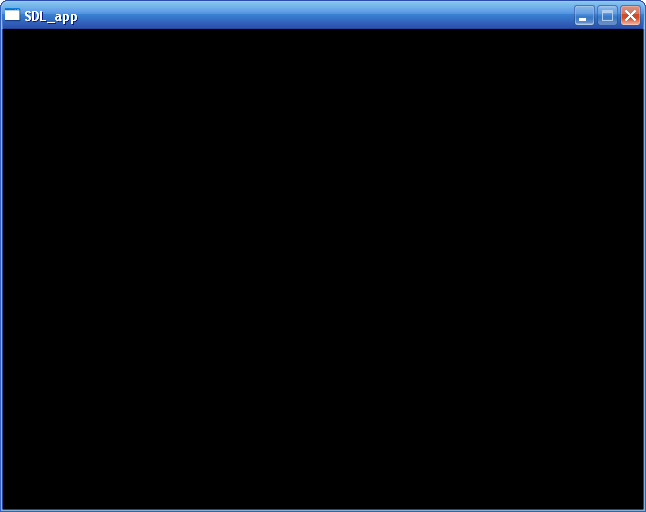
\includegraphics[width=0.8\textwidth]{Chapter_III-2_Empty-window}
\end{figure}

ها قد وصلنا !

إن أردت، قم بوضع العَلم الذي يسمح بتعديل مقاييس النافذة. للعِلْم، في ألعاب الفيديو نفضّل النوافذ ذات الأبعاد الثابتة (لأنه يسهل التعامل معها)، إذا فلنترك النافذة ثابتة كما هي الآن.

\begin{warning}
احذر من العَلَم 
\InlineCode{SDL\_FULLSCREEN}
الخاص بوضع الشاشة الكاملة، و من العَـلم 
\InlineCode{SDL\_NOFRAME}
الذي يقوم بإخفاء حواشي النافذة. بما أنّه لن يكون هناك شريط للعنوان، فلن نكون قادرين على الخروج من البرنامج، إلا بالاستعانة بالمعالج !\\
تريّث قليلاً حتى نتعلّم معالجة الأحداث (في الفصول القادمة) و ستتمكن بعدها من الخروج من النافذة بطريقة أقل عنفاً من استدعاء المعالج.
\end{warning}

\subsection{تغيير عنوان النافذة}

لحدّ الآن، النافذة أخذت عنوانا تلقائيا (و هو 
\InlineCode{SDL\_app}
في الصورة السابقة).\\
هل تريد تغييره ؟

إن الأمر بسيط للغاية، يكفي استعمال الدالة
\InlineCode{SDL\_WM\_SetCaption}.\\
هذه الدالة تأخذ معاملين : المعامل الأول هو العنوان الذي تريد إعطاءه للنافذة، و المعامل الثاني هو العنوان الذي تريد إعطاءه للأيقونة.

خلافاً لما يعتقده الجميع، تغيير اسم الأيقونة لا يعني تغيير صورة الأيقونة التي تظهر أعلى يسار النافذة. هذا لا يعمل دائما (حسب معرفتي، قد يعطي نتائج على الـ\textenglish{GNU/Linux}
في بيئة الـ\textenglish{Gnome}).
شخصياً، أنا أبعث القيمة
\InlineCode{NULL}
إلى الدالة. على أية حال، يمكننا تغيير شكل الأيقونة التي تظهر أعلى يسار النافذة، لكننا سنتعلّم ذلك في الفصل القادم، لأنّ هذا الأمر ليس بمستواك بعد.

هذه نفس الـ\InlineCode{main}
السابقة، مع إضافة الدالة
\InlineCode{SDL\_WM\_SetCaption} :

\begin{Csource}
int main(int argc, char *argv[])
{
	SDL_Init(SDL_INIT_VIDEO);
	SDL_SetVideoMode(640, 480, 32, SDL_HWSURFACE);
	SDL_WM_SetCaption("My super SDL window !", NULL);
	pause();
	SDL_Quit();
	return EXIT_SUCCESS;
}
\end{Csource}

\begin{information}
لاحظ بأنني استعملت القيمة 
\InlineCode{NULL}
للمعاملات غير المهمة بشكل كبير. بالنسبة للـ\textenglish{C}،
يجب أن يتم إعطاء قيم لكل المعاملات التي تستقبلها الدوال، حتى لو كانت هذه المعاملات غير مهمة لك، فأعطها
\InlineCode{NULL}
كما فعلت أنا هنا. بينما الـ\textenglish{C++}
تسمح بألا نعطي أساساً قيمة لبعض المعاملات الاختياريّة عندما نستدعي الدوال.
\end{information}

للنافذة الآن عنوان.

\begin{figure}[H]
	\centering
	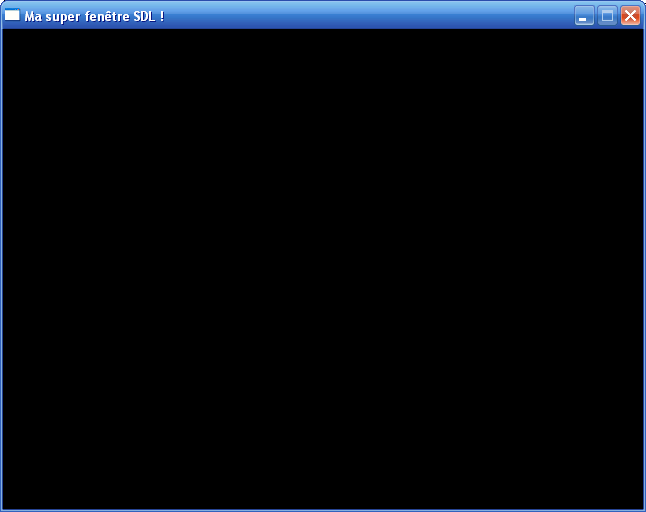
\includegraphics[width=0.8\textwidth]{Chapter_III-2_Window-title}
\end{figure}

\section{التعامل مع المساحات}

لحد الآن تمكّنا من فتح نافذة ذات خلفيّة سوداء. ما نريد الآن هو أن نملأها ببعض الأشياء، أي أن "نرسم" فيها.

كما قلت لك في الفصل السابق، فإن المكتبة
\textenglish{SDL}
هي مكتبة منخفضة المستوى، أي أنها لا توفّر لنا سوى دوال قاعدية، بسيطة جداً.\\
الصراحة هي أن الشكل الوحيد الذي تسمح لنا الـ\textenglish{SDL}
برسمه هو المستطيل ! كلّ ما سنقوم به هو جمع بعض المستطيلات في نافذة. نسمّي هذه المستطيلات بـ\textbf{المساحات}
(\textenglish{Surfaces})،
المساحة هي الوحدة الرسومية القاعدية في الـ\textenglish{SDL}.

\begin{information}
إنه من الممكن أن نرسم أشياء أخرى، مثل الدوائر و المثلثات، إلخ. و لكن لكي نفعل ذلك، يجب أن نكتب بأنفسنا الدوال الّتي تمكّن من فعل ذلك، برسم تلك الأشكال بيكسلا ببيكسل، و إما أن نستعمل مكتبة أخرى إلى جانب الـ\textenglish{SDL}.
الأمر معقّد نوعاً ما، لكن لا تقلق، ستجد بأننا لسنا بحاجة إلى كلّ هذا في التطبيق.
\end{information}

\subsection{مساحتك الأولى : الشاشة}

في كل برامج الـ\textenglish{SDL}،
توجد على الأقل مساحة عمل واحدة و هي ما نسميه بالشاشة 
(\textenglish{Screen})،
و هي مساحة توافق كل النافذة، أي كلّ المساحة السوداء التي تظهر بالنافذة.

في الشفرة المصدرية، كل مساحة يتم تخزينها في متغير من نوع
\InlineCode{SDL\_Surface}.
نعم، إنه نوع بيانات تم إنشاؤه من طرف الـ\textenglish{SDL}
(هذا المتغير عبارة عن هيكل).

بما أن أول مساحة ننشئها هي الشاشة، فهيا بنا :

\begin{Csource}
SDL_Surface *screen = NULL;
\end{Csource}

تلاحظ أنني قمت بإنشاء مؤشّر. لماذا أفعل هذا ؟ لأن الـ\textenglish{SDL}
هي من ستقوم بحجز مكان في الذاكرة من أجل مساحتنا. المساحة بالفعل ليس لها بالضرورة دائما نفس الحجم و لهذا فعلى الـ\textenglish{SDL}
أن تقوم بحجز حيّ من أجلنا (هنا، هذا يعتمد على حجم النافذة التي فتحناها).

لم أقل لك هذا من قبل، لكن الدالة
\InlineCode{SDL\_SetVideoMode}
تقوم بإرجاع قيمة ! ستقوم بإرجاع مؤشّر نحو المكان بالذاكرة المخصص لمساحة الشاشة.\\
ممتاز، يمكننا إذا استرجاع المؤشّر في المتغير 
\InlineCode{screen} :

\begin{Csource}
screen = SDL_SetVideoMode(640, 480, 32, SDL_HWSURFACE);
\end{Csource}

المؤشّر الآن يمكن أن يساوي إحدى القيمتين :

\begin{itemize}
	\item \InlineCode{NULL} :
	المتغير 
	\InlineCode{screen}
	سيساوي
	\InlineCode{NULL}
	إذا فشلت الدالة
	\InlineCode{SDL\_SetVideoMode}
	في تحميل أسلوب العرض الذي تم طلبه. و هذا يحصل حينما يتم اختيار دقة جد عالية أو عدد كبير جداً من الألوان، أكبر من أقصى عدد يتحمله جهازك.
	\item قيمة أخرى : إذا كانت القيمة مختلفة عن 
	\InlineCode{NULL}،
	فهذا يعني أن الـ\textenglish{SDL}
	قامت بحجز المكان، كل شيء على ما يرام !
\end{itemize}

إنه من المستحسن هنا أن تتم معالجة الأخطاء، تماما مثلما فعلنا حينما أردنا تحميل الـ\textenglish{SDL}،
هاهي إذا الدالة

الكاملة بإضافة معالجة الأخطاء للـ\InlineCode{SDL\_SetVideoMode}.

\begin{Csource}
int main(int argc, char *argv[])
{
	SDL_Surface *screen = NULL; // The pointer which stores the surface of the screen
	SDL_Init(SDL_INIT_VIDEO);
	screen = SDL_SetVideoMode(640, 480, 32, SDL_HWSURFACE); // We try to open the window
	if (screen  == NULL) // If we can't, we note it and we exit.
	{
		fprintf(stderr, "Impossible to load the video mode : %s\n", SDL_GetError());
		exit(EXIT_FAILURE);
	}
	SDL_WM_SetCaption("My super SDL window !", NULL);
	pause();
	SDL_Quit();
	return EXIT_SUCCESS;
}
\end{Csource}

الرسالة التي تتركها لنا الدالة
\InlineCode{SDL\_GetError}،
مفيدة من أجل معرفة ما الّذي لم يعمل.

\begin{information}
حكاية صغيرة : مرة أخطأت بينما أردت أن أفتح نافذة بأسلوب الشاشة الكاملة 
(\textenglish{Full screen})،
في عوض أن أطلب الدقة
$1024 \times 768$
كتبت بالخطأ 
$10244 \times 768$،
لم أفهم لماذا لم يتم التحميل، لأنّي لم أنتبه إلى أنني كتبت 4 مرّتين (ربما كنت متعباً). و لحل المشكل ألقيتُ نظرة على الملف 
\InlineCode{stderr.txt}،
توجهت إلى رسالة الخطأ و اكتشفت بأن الدقة التي طلبتها مرفوضة (شيء يثير الفضول أليس كذلك~؟).
\end{information}

\subsection{تلوين مساحة}

لا توجد 36 طريقة لملء مساحة، الحقيقة أنه توجد طريقتان :

\begin{itemize}
	\item إما أن يتم تلوين المساحة بلون موحّد.
	\item إما أن يتم ملؤها عن طريق تحميل صورة.
\end{itemize}

\begin{information}
يمكنك في الحقيقة الرسم في المساحة بيكسلا ببيكسل، لكن هذه الطريقة معقّدة، لن نراها هنا.
\end{information}

سنرى أولا كيف نقوم بتلوين مساحة بلون موحّد. في الفصل القادم سنتعلّم كيف نقوم بتحميل صورة.

الدالة التي تسمح بتلوين النافذة بلون موحّد هي
\InlineCode{SDL\_FillRect}
(العبارة 
\InlineCode{FillRect}
تعني ملء مستطيل بالإنجليزيّة). هذه الدالة تستقبل 3 معاملات و هي :

\begin{itemize}
	\item مؤشّر نحو المساحة التي نريد التلوين عليها (مثلا
	\InlineCode{screen}).
	\item الجزء من المساحة الذي نريد تلوينه، إذا أردت تلوين كل المساحة (و هذا الّذي نريده) فلتكن قيمة المؤشر 
	\InlineCode{NULL}.
	\item اللون الذي نريد أن نلوّن به المساحة.
\end{itemize}

كملخّص :

\begin{Csource}
SDL_FillRect(surface, NULL, color);
\end{Csource}

\subsubsection{التحكم في الألوان بالـ\textenglish{SDL}}

في الـ\InlineCode{SDL}
كل لون مخزن في عدد من نوع
\InlineCode{Uint32}.

\begin{question}
إذا كان عدداً، لماذا إذا لم نستعمل ببساطة النوع
\InlineCode{int}
أو النوع
\InlineCode{long} ؟
\end{question}

الـ\InlineCode{SDL}
هي مكتبة متعددة المنصات، و كما تعلم فحجم الـ\InlineCode{int}
يتغير من نظام تشغيل إلى آخر. لهذا فإن الـ\InlineCode{SDL}
تقوم باستخدام أعداد من أنواع جديدة، هذه الأنواع الجديدة تحجز نفس المكان بالذاكرة في كل أنظمة التشغيل.\\

هناك مثلاً :

\begin{itemize}
	\item \InlineCode{Uint32} :
عدد صحيح بحجم
\textenglish{32 bits}
أي
\textenglish{4 octets}
(للتذكير :
\textenglish{1 octet = 8 bits}).
	\item \InlineCode{Uint16} :
عدد صحيح مشفر على
\textenglish{16 bits} (\textenglish{2 octets}).
	\item \InlineCode{Uint8} :
عدد طبيعي مشفر على
\textenglish{8 bits} (\textenglish{1 octet}).
\end{itemize}
لن تستعمل المكتبة سوى
\InlineCode{typedef}
لتقوم بتغيير قيمة العدد على حسب نظام التشغيل. إذا كنت فضولياً، فألق نظرة على الملف
\InlineCode{SDL\_types.h}.

لن نتأخر في التعامل مع كل هذا، فالتفاصيل لا تهم حالياً. كل ما عليك تذكره هو أن النوع
\InlineCode{Uint32}
لا يخزن إلا عددا صحيحاً ليس إلا، مثل
\InlineCode{int}.

\begin{question}
لكن كيف أعرف أي عدد يوافق اللون الّذي أريد ؟
\end{question}

هناك بالفعل دالة من أجل ذلك :
\InlineCode{SDL\_MapRGB}،
هذه الأخيرة تستقبل 4 معاملات :

\begin{itemize}
	\item صيغة الألوان : هذه الصيغة تعتمد على عدد
	\textenglish{bits/pixel}
	التي قد طلبتها بالـ\InlineCode{SDL\_SetVideoMode}.
	يمكنك استرجاع القيمة فهي موجودة في المتغير الداخلي
	\InlineCode{screen->format}.
	\item كمية الأحمر في اللون.
	\item كمية الأخضر في اللون.
	\item كمية الأزرق في اللون.
\end{itemize}

قد لا يعرف البعض بأن كل الألوان يتم تشكيلها عن طريق خلط الألوان : أزرق، أحمر و أخضر.\\
كل كمية تتدرج من العدد 0 (لا يوجد لون) إلى العدد 255 (كل اللون موجود). أي أننا لو كتبنا :

\begin{Csource}
SDL_MapRGB(screen->format, 255, 0, 0)
\end{Csource}

فاللون المتشكل سيكون أحمرا. لا وجود للأخضر و لا للأزرق، أما لو نكتب :
\begin{Csource}
SDL_MapRGB(screen->format, 0, 0, 255)
\end{Csource}
اللون سيكون أزرقا، بينما لو نكتب :
\begin{Csource}
SDL_MapRGB(screen->format, 255, 255, 255)
\end{Csource}

اللون سيكون أبيضا لأننا دمجنا كل الألوان، لو أنك تريد تشكيل اللون الأسود، فلتجعل كل القيم على 0.

\begin{question}
ألا يمكننا استعمال لون آخر غير هذه الألوان ؟
\end{question}

كلّا، يمكنك ذلك لو أنك تقوم بمزج الألوان بشكل ذكي. للمساعدة في ذلك، توجه إلى برنامج
\textenglish{Paint}
ثم إلى
\InlineCode{Colors} / \InlineCode{Modify the colors}،
انقر على
\InlineCode{Define the colors}
ثم
\InlineCode{Custom}.\\
هنا، اختر اللون الّذي يلائمك. أنظر إلى الصورة التالية :

\begin{figure}[H]
	\centering
	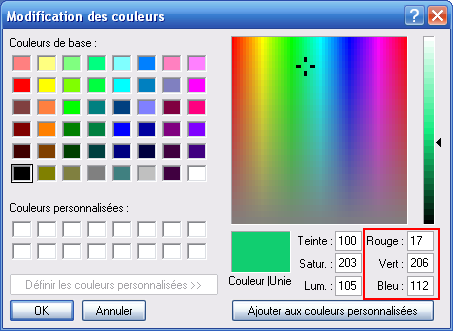
\includegraphics[width=0.7\textwidth]{Chapter_III-2_Colors}
\end{figure}

مركّبات اللون متواجدة في أسفل يمين النافذة. كما ترى فقد اخترت لونا أخضر مزرقّا، و هو يتكوّن من 17 من الأحمر، 206 من الأخضر، و 112 من الأزرق.
\subsubsection{تلوين الشاشة}

الدالة
\InlineCode{SDL\_MapRGB}
تقوم بإرجاع عدد من نوع
\InlineCode{Uint32}
يوافق اللّون المختار.\\
يمكننا إذا تعريف متغير باسم
\InlineCode{blueGreen}
يحوي الشفرة الخاصة لاسترجاع هذا اللون :

\begin{Csource}
Uint32 blueGreen = SDL_MapRGB(screen->format, 17, 206, 112);
\end{Csource}

ليس من الضروري المرور دائما على متغير لتخزين اللون المراد استعماله (إلا إن كنت تحتاجه فعلا في برنامجك).\\
يمكنك مباشرة إعطاء القيمة التي تم ارجاعها من طرف الدالة
\InlineCode{SDL\_MapRGB}
إلى الدالة
\InlineCode{SDL\_FillRect}.

لو نريد أن نملأ الشاشة باللون الأخضر المزرق، يمكننا كتابة :

\begin{Csource}
SDL_FillRect(screen , NULL, SDL_MapRGB(screen->format, 17, 206, 112));
\end{Csource}

لقد قمنا باستدعاء دالة خلال استدعاء دالة أخرى، أعتقد أنك تعرف بأن الأمر ممكن و لا يسبب أيّ مشاكل في لغة
\textenglish{C}.

\subsubsection{تحديث الشاشة}

لقد اقتربنا من تحقيق الهدف.\\
لقد نسينا أمراً بسيطاً : و هو الأمر بتحديث الشاشة. بالفعل، فالأمر 
\InlineCode{SDL\_FillRect}
يقوم بتلوين الشاشة، لكن هذا لا يحصل إلا في الذاكرة، إذ يجب أن نطلب من الحاسوب تحديث الشاشة لاستعمال البيانات الجديدة.

من أجل هذا سنستعمل الدالة 
\InlineCode{SDL\_Flip}،
سنتكلم بشكل مفصل عن هذه الدالة لاحقا.\\
الدالة تستقبل معاملا واحدا و هو الشاشة
\InlineCode{screen}.

\subsubsection{فلنلخّص كل شيء !}

هذه دالة
\InlineCode{main}
تقوم بفتح نافذة ملونة باللون الأخضر المزرق :

\begin{Csource}
int main(int argc, char *argv[])
{
	SDL_Surface *screen = NULL;
	SDL_Init(SDL_INIT_VIDEO);
	screen = SDL_SetVideoMode(640, 480, 32, SDL_HWSURFACE);
	SDL_WM_SetCaption("My super SDL window !", NULL);
	// We colorize the screen with blue-green color
	SDL_FillRect(screen, NULL, SDL_MapRGB(screen->format, 17, 206, 112));
	SDL_Flip(screen); 
	pause();
	SDL_Quit();
	return EXIT_SUCCESS;
}
\end{Csource}

هاهي النتيجة :

\begin{figure}[H]
	\centering
	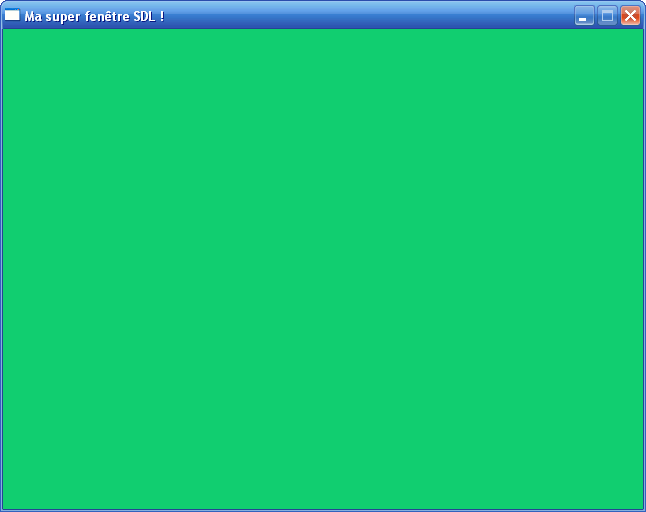
\includegraphics[width=0.8\textwidth]{Chapter_III-2_Window-color}
\end{figure}

\subsection{رسم مساحة أخرى في الشاشة}

النتيجة السابقة جيدة، لكننا لن نتوقف هنا. لحد الآن ليست لدينا سوى مساحة واحدة و هي الشاشة. نحن نريد أن نقوم بالرسم عليها، أي "نلصق" مساحات أخرى عليها بألوان مختلفة.

لهذا يجب علينا إنشاء متغير من نوع
\InlineCode{SDL\_Surface}
للمساحة الجديدة :

\begin{Csource}
SDL_Surface *rectangle = NULL;
\end{Csource}

سنطلب إذا من الـ\InlineCode{SDL}
أن تقوم بحجز مكان في الذاكرة من أجل المساحة الجديدة.\\
من أجل الشاشة كنا قد استعملنا
\InlineCode{SDL\_SetVideoMode}.
لكن هذه الأخيرة لا تعمل إلا على  الشاشة (المساحة الرئيسية)، لا نريد أن نقوم بإنشاء نافذة من أجل كل مستطيل نريد إنشاءه !

توجد إذا دالة أخرى من أجل إنشاء مساحة : 
\InlineCode{SDL\_CreateRGBSurface}.
هذه هي التي سنقوم باستعمالها في كل مرة نريد أن ننشئ مساحة جديدة.

هذه الدالة تستقبل العديد من المعاملات (ثمانية !). لكنني لن أتطرّق إلا للمعاملات التي تهمّنا لحدّ الآن.\\
بما أن لغة 
\textenglish{C}
تُلزمنا بإدخال قيم لكل المعاملات، فإننا سنقوم بوضع القيمة 0 في مكان كل معامل لا يهمّنا.

فلنتأمل قليلا في المعاملات الأربع الأولى (يجدر بها أن تذكّرنا بإنشاء الشاشة).

\begin{itemize}
	\item قائمة الأعلام (الخيارات). لديك الاختيار بين :
	\begin{itemize}
		\item \InlineCode{SDL\_HWSURFACE} :
		المساحة يتم تحميلها في الذاكرة الرسوميّة. و هي تحتوي على مكان أقل مقارنة بالذاكرة الخاصة بالنظام (حقيقة، مع بطاقات الـ\textenglish{3D}
		في أيامنا هذه، قد لا يكون لهذا تأثير)، لكنها ذاكرات سريعة و فعّالة.
		\item \InlineCode{SDL\_SWSURFACE} :
		يتم تحميل المساحة في الذاكرة الخاصة بالنظام، أين يوجد الكثير من المكان، لكن هذا الاختيار سيجبر المعالج على القيام بحسابات أكثر. لو أنك حمّلت المساحة على الذاكرة الرسوميّة، فإن البطاقة 
		\textenglish{3D}
		هي المسؤولة عن القيام بأغلب الحسابات.
	\end{itemize}
	\item عرض المساحة (\textenglish{pixels}).
	\item ارتفاع المساحة (\textenglish{pixels}).
	\item عدد الألوان (\textenglish{bits/pixel}).
\end{itemize}

هكذا إذا نقوم بحجز مكان للمساحة الجديدة في الذاكرة :

\begin{Csource}
rectangle = SDL_CreateRGBSurface(SDL_HWSURFACE, 220, 180, 32, 0, 0, 0, 0);
\end{Csource}

الأربع معاملات الأخيرة تساوي 0، كما قلت لك، لأننا لا نهتم بأمرها حالياً. 

بما أننا قمنا بالحجز اليدوي للذاكرة، فيجب علينا تحريرها باستعمال الدالة 
\InlineCode{SDL\_FreeSurface}
و التي نستعملها قبل 
\InlineCode{SDL\_Quit} :

\begin{Csource}
SDL_FreeSurface(rectangle);
SDL_Quit();
\end{Csource}

\begin{information}
ليس هناك من داعٍ إلى تحرير المساحة
\InlineCode{screen}
باستعمال
\InlineCode{SDL\_FreeSurface}
لأنه يتم تحريرها تلقائياً عند استدعاء
\InlineCode{SDL\_Quit}.
\end{information}

يمكننا الآن تلوين المساحة الجديدة باللون الأبيض مثلا :

\begin{Csource}
SDL_FillRect(rectangle, NULL, SDL_MapRGB(screen->format, 255, 255, 255));
\end{Csource}

\subsubsection{لصق المساحة بالشاشة}

اقتربنا من النهاية، هيا بعض الشجاعة ! المساحة جاهزة، لكن لو تحاول تجريب البرنامج، ستلاحظ أنها لن تظهر على الشاشة، بالفعل إذ أن المساحة
\InlineCode{screen}
هي وحدها التي تم إظهارها. لكي نستطيع رؤية مساحتنا الجديدة يجب أن نقوم بـ\textbf{تسوية}
المساحة، أي لصقها على الشاشة، سنستعمل لأجل هذا الدالة 
\InlineCode{SDL\_BlitSurface}.
 هذه الدالة تنتظر :
 
\begin{itemize}
	\item المساحة التي نريد لصقها (هنا 
	\InlineCode{rectangle}).
	\item معلومة حول الجزء من تلك المساحة الذي نريد لصقه (اختياري). لن يهمنا الأمر الآن فنحن نريد لصق كل المساحة و لهذا فستكون القيمة
	\InlineCode{NULL}.
	\item المساحة التي نريد أن نلصق عليها المساحة الجديدة (في حالتنا هذه نتكلم عن الشاشة 
	\InlineCode{screen}).
	\item مؤشّر نحو متغير يحتوي الإحداثيّات. هذه الإحداثيات تشير إلى المكان الذي نريد أن نلصق عليه المساحة، أي موقعه.
	
للإشارة إلى الإحداثيّات، نحتاج إلى استعمال متغير من نوع 
\InlineCode{SDL\_Rect}.\\
إنّه هيكل يحتوي العديد من المركّبات، إثنتان منها تهمّنا :
	\begin{itemize}
		\item \InlineCode{x} : 
الفاصلة.
		\item \InlineCode{y} : 
الترتيبة. 
	\end{itemize}	
\end{itemize}

يجب أن تعرف أن الإحداثيّة
\InlineCode{(0, 0)}
توافق أقصى نقطة في يسار أعلى الشاشة.\\
أما الإحداثيّة 
\InlineCode{(640, 480)}
فهي توافق النقطة الموجودة في أقصى يمين أسفل الشاشة، و هذا إن كنت قد فتحت نافذة بحجم
$640 \times 480$
مثلي.

هذا المخطط سيساعدك في الفهم  :

\begin{figure}[H]
	\centering
	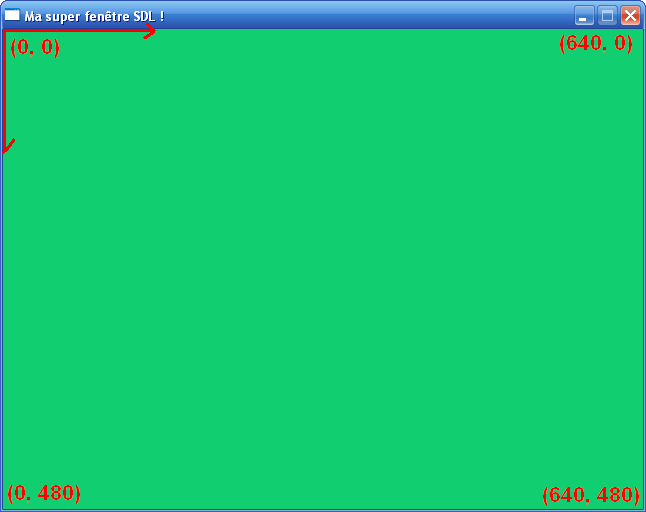
\includegraphics[width=0.8\textwidth]{Chapter_III-2_Window-coordinates}
\end{figure}

إذا كنت قد درست الرياضيات من قبل، فعلى الأرجح لن تضيع بينما تحاول  فهم كيفية العمل. فلننشئ إذا متغيرا 
\InlineCode{position}.
سنعطي القيمة 0 لكل من الفاصلة و الترتيبة و ذلك ليتم لصق مساحتنا (المستطيل) في أعلى يسار النافذة :

\begin{Csource}
SDL_Rect position;
position.x = 0;
position.y = 0;
\end{Csource}

و الآن بما أننا حددنا موقعنا في النافذة، يمكننا تسوية المساحة الجديدة على الشاشة :

\begin{Csource}
SDL_BlitSurface(rectangle, NULL, screen, &position);
\end{Csource}
 
لاحظ أنني استعملت الرمز
\InlineCode{\&}
و ذلك لأنه يجب علينا إرسال عنوان المتغير
\InlineCode{position}.

\subsubsection{تلخيص الشفرة المصدرية}

أعتقد أن وضع الشفرة المصدرية الّتي تلخص ما شرحته لن يكون مضراً :

\begin{Csource}
int main(int argc, char *argv[])
{
	SDL_Surface *screen = NULL, *rectangle = NULL;
	SDL_Rect position;
	SDL_Init(SDL_INIT_VIDEO);
	screen = SDL_SetVideoMode(640, 480, 32, SDL_HWSURFACE);
	// Surface allocation
	rectangle = SDL_CreateRGBSurface(SDL_HWSURFACE, 220, 180, 32, 0,0, 0, 0);
	SDL_WM_SetCaption("My super SDL window !", NULL);
	SDL_FillRect(screen, NULL, SDL_MapRGB(screen->format, 17, 206,112));
	position.x = 0; // The coordinates of the surface will be (0, 0)
	position.y = 0;
	// Filling the surface with white color
	SDL_FillRect(rectangle, NULL, SDL_MapRGB(screen->format, 255,255, 255));
	SDL_BlitSurface(rectangle, NULL, screen, &position); // Sticking the surface on the screen 
	SDL_Flip(screen); // Updating the screen
	pause();
	SDL_FreeSurface(rectangle); // Freeing the surface
	SDL_Quit();
	return EXIT_SUCCESS;
}
\end{Csource}

شاهد النتيجة :

\begin{figure}[H]
	\centering
	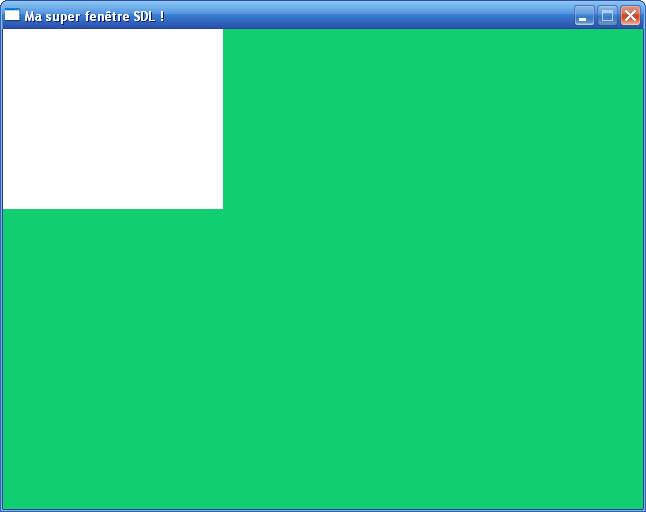
\includegraphics[width=0.8\textwidth]{Chapter_III-2_Colors-paste}
\end{figure}

\subsubsection{مركزةُ المساحة في الشاشة}

نحن نجيد إظهار المساحة في أعلى اليسار. يسهل أيضا موقعتها أسفل يمين الشاشة. ستكون الإحداثيات
\mbox{($640 - 220, 480 - 180$)}،
لأنه يجب إنقاص حجم المستطيل ليتم إظهاره كاملا. 

لكن كيف تتم مركزةُ المستطيل الأبيض ؟ لو تفكّر قليلاً ستجد بأن الحساب
\textit{رياضياتيّ}.
فهنا نعرف الهدف من الرياضيات و الحساب الهندسي !\\
كلّ هذا الأمر بمستوى سهل هنا :

\begin{Csource}
position.x = (640 / 2) - (220 / 2);
position.y = (480 / 2) - (180 / 2);
\end{Csource}

فاصلة المستطيل هي نصف عرض الشاشة
($640 / 2$).
و لكن، بالإضافة إلى هذا، يجب أن يتم إنقاص نصف طول المستطيل أيضاً 
($220 / 2$)،
لأنك إن لم تنقص هذا الحجم، سيكون تمركز المستطيل خاطئاً (جرّب عدم فعل ذلك و ستفهم ما الّذي أعنيه).\\
كذلك بالنسبة للترتيبة مع ارتفاع الشاشة و المستطيل.

النتيجة : المستطيل الأبيض يتمركز بشكل جيد في الشاشة.

\begin{figure}[H]
	\centering
	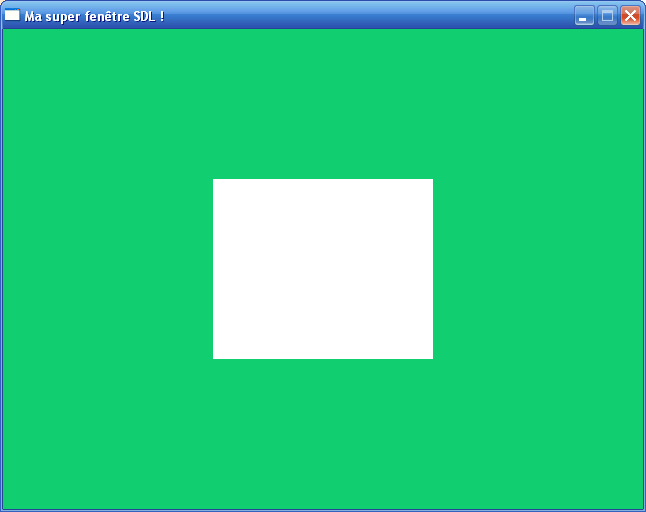
\includegraphics[width=0.8\textwidth]{Chapter_III-2_Window-color-centered}
\end{figure}

\section{تمرين : إنشاء تدرّج لونيّ}

سننهي الفصل بتمرين صغير (مصحّح) متبوع بسلسلة تمارين أخرى (غير مصححة من أجل حثّك على التدريب).

التمرين المصحح ليس صعباً حقّا : ما نريد إنشاءه هو نافذة متدرّجة الألوان عموديا من الأسود إلى الأبيض.\\
سيكون عليك إنشاء 255 مساحة بارتفاع 1 بيكسل. كل مساحة لها لون مختلف أكثر فأكثر سوادا.

هذا ما يجب عليك الحصول عليه في النهاية، صورة مشابهة لهذه :

\begin{figure}[H]
	\centering
	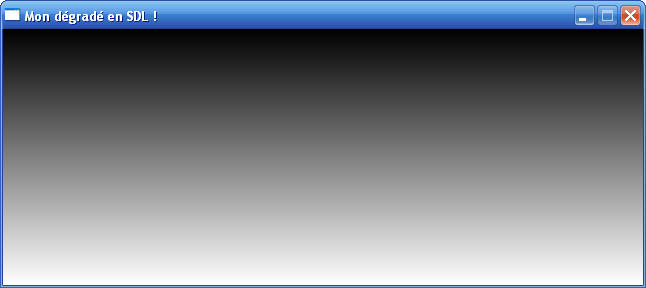
\includegraphics[width=0.8\textwidth]{Chapter_III-2_Window-gradient}
\end{figure}

 إنه أمر جميل، أليس كذلك ؟ الشيء الأجمل هو أن بعض الحلقات التكرارية كافية من أجل تحقيق المطلوب.
 
لفعل ذلك يجب إنشاء 256 مساحة (أي 256 سطر) تحتوي مركبات الألوان (أحمر، أخضر، أزرق) التالية~:

\begin{Csource}
0, 0, 0) // Black
(1, 1, 1) // Gray that is so so close from black
(2, 2, 2) // Gray that is so close from black
...
(128, 128, 128) // Medium gray (to 50 %)
...
(253, 253, 253) // Gray that is so  close from white
(254, 254, 254) // Gray that is so so close from white
(255, 255, 255) // White
\end{Csource}

يجب على أيّ كان أن يعرف أنّه بحاجة إلى حلقة تكراريّة للقيام بهذا (لن تسعد بتكرار 256 سطرا !). و لهذا سنقوم بإنشاء جدول من نوع 
\InlineCode{SDL\_Surface*}
من 256 خانة.

إلى العمل. لديك 5 دقائق !

\subsection{تصحيح !}
 
يجب أولا أن نقوم بتعريف جدول من 256
\InlineCode{SDL\_Surface*}.
سنهيّؤه على
\InlineCode{NULL} :

\begin{Csource}
SDL_Surface *lines[256] = {NULL};
\end{Csource}

سنعرف متغيراً
\InlineCode{i}
من أجل الحلقات 
\InlineCode{for}.

سنغيّر أيضاً ارتفاع النافذة لكي تكون مناسبة للعمل. إذ سنعطيها 256 بيكسلز كارتفاع، و ذلك من أجل عرض كل سطر من بين 256 سطرا.

سنستعمل بعد ذلك حلقة تكرارية
\InlineCode{for}
من أجل حجز مكان لـ256 مساحة الّتي تم إنشاؤها. الجدول سيستقبل 256 مؤشّرا إلى كلّ واحد من المساحات المنشأة :

\begin{Csource}
for (i = 0 ; i <= 255 ; i++)
	lines[i] = SDL_CreateRGBSurface(SDL_HWSURFACE, 640, 1, 32, 0,0, 0, 0);
\end{Csource}

بعد ذلك نقوم بملء و لصق كل مساحة في الشاشة واحدة بواحدة.

\begin{Csource}
for (i = 0 ; i <= 255 ; i++)
{
	position.x = 0; // The lines are to the left (0 abscissa)
	position.y = i; // The vertical position depends on the line's number
	SDL_FillRect(lines[i], NULL, SDL_MapRGB(screen->format, i, i, i)); // Drawing
	SDL_BlitSurface(lines[i], NULL, screen, &position); // Sticking
}
\end{Csource}

 لاحظ أنني استعمل كل الوقت المتغير 
\InlineCode{position}.
إذ ليس لازما أن ننشئ 256 واحدا، لأننا لن نقوم إلا ببعث المتغير إلى الدالة 
\InlineCode{SDL\_BlitSurface}.
يمكننا إذن إعادة استخدامه دون مشاكل.\\
في كلّ مرة أقوم بالتعديل على الترتيبة
(\InlineCode{y})،
لتسوية المساحة على الارتفاع الصحيح. اللون يعتمد في كلّ مرة على قيمة المتغير
\InlineCode{i}
(ستكون
$0, 0, 0$
في أوّل مرّة و $255, 255, 255$ في آخر مرّة).

\begin{question}
لكن لماذا قيمة 
\InlineCode{x}
هي 0 دائماً ؟\\
كيف يمكن للمساحة أن تتلون كليا إذا كانت قيمة الـ\InlineCode{x}
دائما 0 ؟
\end{question}

المتغير
\InlineCode{position}
يشير إلى أي مكان تتواجد فيه المنطقة أعلى اليسار (هنا نتكلم عن السطر). هي لا تحدد عرض المساحة و إنما فقط أين تتواجد المركّبة على الشاشة.\\
بما أن كل الأسطر تبدأ في أقصى يسار النافذة، فستكون الفاصلة مساوية لـ0. حاول وضع فاصلة تساوي 50 لترى ماذا سيعطيك : كل الأسطر ستتنحي إلى اليمين.\\
بما أن المساحة تأخذ 640 بيكسل كطول ، فإن الـ\textenglish{SDL}
تقوم بإنشاء 640 بيكسلا في اتجاه اليمين (من نفس اللون) إنطلاقاً من المركبات التي يشير إليها المتغير 
\InlineCode{position}.

في المخطط التالي أريك مركبات النقطة المتواجدة أعلى يسار الشاشة (وضعية أول سطر) ومركبات النقطة المتواجدة أسفل يسار الشاشة (وضعية آخر سطر).

\begin{figure}[H]
	\centering
	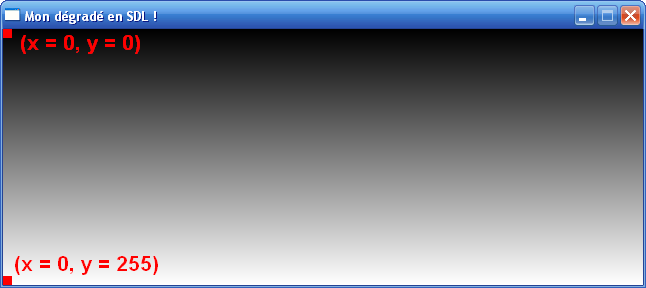
\includegraphics[width=0.8\textwidth]{Chapter_III-2_Window-gradient-coordinates}
\end{figure}

كما ترى، من الأعلى إلى الأسفل، المحور لا يتغير 
(\InlineCode{x}
يبقى مساويا لـ0) بينما 
\InlineCode{y}
وحده يتغير من أجل كل سطر جديد، و بهذا 
\InlineCode{position.y = i;}.

أخيراً لا تنس أنه يجب تحرير الذاكرة من أجل كل مساحة من الـ256 مساحة المنشأة، بمساعدة حلقة بالطبع.

\begin{Csource}
for (i = 0 ; i <= 255 ; i++) // Don't forget to free the 256 surfaces
	SDL_FreeSurface(lines[i]);
\end{Csource}

\subsubsection{ملخّص \texttt{main}}

هذه هي الدالة
\InlineCode{main}
كاملة :

\begin{Csource}
int main(int argc, char *argv[])
{
	SDL_Surface *screen = NULL, *lines[256] = {NULL};
	SDL_Rect position;
	int i = 0;
	SDL_Init(SDL_INIT_VIDEO);
	screen = SDL_SetVideoMode(640, 256, 32, SDL_HWSURFACE);
	for (i = 0 ; i <= 255 ; i++)
		lines[i] = SDL_CreateRGBSurface(SDL_HWSURFACE, 640, 1, 32,0, 0, 0, 0);
	SDL_WM_SetCaption("My SDL gradient !", NULL);
	SDL_FillRect(screen , NULL, SDL_MapRGB(screen ->format, 0, 0, 0));
	for (i = 0 ; i <= 255 ; i++)
	{
		position.x = 0; // The lines are to the left
		position.y = i; // The vertical position depends on the line's number
		SDL_FillRect(lines[i], NULL, SDL_MapRGB(screen->format, i, i, i));
		SDL_BlitSurface(lines[i], NULL, screen, &position);
	}
	SDL_Flip(screen);
	pause();
	for (i = 0 ; i <= 255 ; i++) // Don't forget to free the 256 surfaces
		SDL_FreeSurface(lines[i]);
	SDL_Quit();
	return EXIT_SUCCESS;
}
\end{Csource}

{\large"أريد تمارين للتدريب !"}

لا مشكلة، مولّد التمارين مُشَغّل !

\begin{itemize}
	\item قم بإنشاء تدرج عكسي للألوان، أي من الأبيض للأسود. هذا الأمر لن يكون صعبا للبدأ !
	\item يمكنك أيضاً وضع كلى التدرّجين، من الأبيض للأسود ثم من الأسود للأبيض (ستأخذ النافذة ضعف الارتفاع الحالي).
	\item أكثر صعوبة قليلا، يمكنك وضع تدرج أفقي بدل التدرج العمودي.
	\item حاول إنشاء تدرج ألوان مختلفة عن الأسود و الأبيض. جرب مثلا من الأحمر إلى الأسود، من الأخضر إلى الأسود، و من الأزرق إلى الأسود، ثمّ من الأحمر إلى الأبيض، إلخ.
\end{itemize}

\section*{ملخّص}

\begin{itemize}
	\item يتم تحميل الـ\InlineCode{SDL}
	بواسطة الـ\InlineCode{SDL\_Init}
	في بداية البرنامج، و يتم إيقافها باستعمال
	\InlineCode{SDL\_Quit}
	في النهاية.
	\item الأعلام هي ثوابت يمكن جمعها فيما بينها باستعمال الرمز 
	\InlineCode{|}،
	 و هي تلعب دور الخواص.
	\item تقوم الـ\textenglish{SDL}
	بالتعامل مع المساحات و التي هي عبارة عن مستطيلات من نوع 
	\InlineCode{SDL\_Surface}.
	الرسم على النافذة يتم بالاستعانة بهذه المساحات.
	\item توجد دائما على الأقل مساحة واحدة و التي تحجز كلّ النافذة، و نسميها في أغلب الأحيان الشاشة 
	(\InlineCode{screen}).
	\item ملء مساحة يتم باستعمال
	\InlineCode{SDL\_FillRect}،
	ولصقها في الشاشة يتم باستعمال
	\InlineCode{SDL\_BlitSurface}.
	\item الألوان معرّفة بمزيج من الأحمر، الأزرق و الأخضر.
\end{itemize}
